We perform the analysis on a dataset corresponding to $1.1\pm0.1\ifb$ integrated luminosity.

Table~\ref{tab:zzselection_all} shows the number of events observed in 
data, comparing to the expected background contribution at the \zz 
preselection level. The background estimation was discussed at Section~\ref{sec:backgrounds}. 
Figure~\ref{fig:zz_0j_1} the distributions of key analysis variables observed in data, comparing 
to the SM expectations from simulation in the 0-jet bin final state.  

%%%%%%%%
\begin{table}[!ht]
\begin{center}
\begin{tabular} {c|c|c|cccc}
\hline
 Jet-Bin & data & all bkg. & peaking-$\WZ$/$\ZZ$ & $\WW$+$\ttbar+tW$ & $\dyll$ & $\Wjets$ \\
\hline
 0-Jet & X & X & X  & X & X & X\\
 1-Jet & X & X & X  & X & X & X\\
% 2-Jet & X & X & X  & X & X & X \\
\hline
\hline
\end{tabular}
\caption{Expected number of signal and background events from the data-driven methods for an 
  integrated luminosity of \intlumi  after applying the $\ZZ$ selection requirements. 
Both statistical and systematic uncertaities are reported. }
   \label{tab:zzselection_all}
  \end{center}
\end{table}
%%%%%%%%

Table~\ref{tab:yield_zzpresel} shows the number of observed events in data after the $\ZZ$ 
selection, compared to the expected number of signal and background events from the data-driven methods for an 
 integrated luminosity of \intlumi  in the 0 and 1 jet bins. 
The MC expectations includes the lepton efficiencies, trigger 
efficiencies, pileup reweighting, higher order reweighting on the $\hzz$ and $\pt$-dependent 
reweighting on $\ZZ$ and the data/simulation scale factors derived in Section~\ref{sec:backgrounds}.  
Tables~\ref{tab:yield_hzz200}-\ref{tab:yield_hzz400} shows the equivalent results 
applying the $\hzz$ ($m_{H}=200,250,300,400\GeVcc$) selections~\ref{sec:signal_selection}.


%%%%%%%%
\begin{table}[!ht]
\begin{center}
\begin{tabular}{c|cc|c}
\hline
sample    & $\mu\mu$   & ee     & TOTAL\\ \hline 
\multicolumn{4}{c} { 0 Jet Bin} \\
\hline
%hww300   & 0.74 $\pm$ 0.03   & 0.55 $\pm$ 0.02   & 1.29 $\pm$ 0.04 \\  
$\wjets$   & 0.00 $\pm$ 0.00   & 1.29 $\pm$ 0.63   & 1.29 $\pm$ 0.63 \\  
\qqww   & 10.91 $\pm$ 0.35   & 7.09 $\pm$ 0.27   & 17.99 $\pm$ 0.45 \\  
\ggww   & 0.68 $\pm$ 0.04   & 0.46 $\pm$ 0.03   & 1.14 $\pm$ 0.05 \\  
\wz   & 7.12 $\pm$ 0.30   & 4.03 $\pm$ 0.22   & 11.15 $\pm$ 0.37 \\  
$\ZZ$   & 14.54 $\pm$ 0.28   & 9.67 $\pm$ 0.22   & 24.21 $\pm$ 0.35 \\  
$\ttbar$   & 1.44 $\pm$ 0.63   & 0.41 $\pm$ 0.25   & 1.85 $\pm$ 0.67 \\  
$\tw$   & 0.63 $\pm$ 0.16   & 0.58 $\pm$ 0.15   & 1.21 $\pm$ 0.22 \\  
$\dytt$   & 0.00 $\pm$ 0.00   & 0.00 $\pm$ 0.00   & 0.00 $\pm$ 0.00 \\  
$\dyll$   & 8.17 $\pm$ 0.10   & 8.17 $\pm$ 0.10   & 16.34 $\pm$ 0.15 \\  
\hline
Background   & 43.49 $\pm$ 0.85   & 31.70 $\pm$ 0.81   & 75.18 $\pm$ 1.17 \\  
hzz300   & 2.50 $\pm$ 0.03   & 1.75 $\pm$ 0.03   & 4.25 $\pm$ 0.04 \\  
\hline
DATA   & 39.00 $\pm$ 6.24   & 31.00 $\pm$ 5.57   & 70.00 $\pm$ 8.37 \\ 
\hline 
\multicolumn{4}{c} { 1 Jet Bin} \\
\hline
$\wjets$   & 0.00 $\pm$ 0.00   & 0.00 $\pm$ 0.00   & 0.00 $\pm$ 0.00 \\  
\qqww   & 3.11 $\pm$ 0.18   & 2.04 $\pm$ 0.14   & 5.15 $\pm$ 0.23 \\  
\ggww   & 0.21 $\pm$ 0.02   & 0.14 $\pm$ 0.02   & 0.34 $\pm$ 0.03 \\  
\wz   & 3.74 $\pm$ 0.22   & 2.50 $\pm$ 0.17   & 6.24 $\pm$ 0.28 \\  
\zz   & 3.68 $\pm$ 0.14   & 2.59 $\pm$ 0.11   & 6.27 $\pm$ 0.18 \\  
$\ttbar$  & 2.35 $\pm$ 0.70   & 2.77 $\pm$ 0.81   & 5.11 $\pm$ 1.07 \\  
\tw   & 0.72 $\pm$ 0.15   & 0.82 $\pm$ 0.17   & 1.54 $\pm$ 0.23 \\  
$\dytt$   & 0.00 $\pm$ 0.00   & 0.00 $\pm$ 0.00   & 0.00 $\pm$ 0.00 \\  
$\dyll$  & 8.79 $\pm$ 0.11   & 8.79 $\pm$ 0.11   & 17.57 $\pm$ 0.15 \\  
\hline
Background   & 22.59 $\pm$ 0.79   & 19.63 $\pm$ 0.87   & 42.22 $\pm$ 1.17 \\  
hzz300   & 1.42 $\pm$ 0.02   & 0.98 $\pm$ 0.02   & 2.40 $\pm$ 0.03 \\  
\hline
DATA   & 21.00 $\pm$ 4.58   & 18.00 $\pm$ 4.24   & 39.00 $\pm$ 6.24 \\ 
\hline
\end{tabular}
\caption{
Expected number of signal and background events from the data-driven methods for an 
  integrated luminosity of \intlumi  after the {\bf $\ZZ$ pre-selection in the 0/1-Jet bin}. 
Only statistical uncertainties are reported. The MC expectations includes the lepton efficiencies, 
trigger efficiencies, pileup reweighting, 
higher order reweighting on the $\hzz$ and $\pt$-dependent reweighting on $\ZZ$. The $\ttbar$, 
$\tw$, $\ww$, $\dytt$ and $\wjets$ yields include the data/MC scale factors derived in section~\ref{sec:backgrounds}. }
\label{tab:yield_zzpresel}
\end{center}
\end{table}
%%%%%%%%


%%%%%%%%
\begin{table}[!ht]
\begin{center}
\begin{tabular}{c|cc|c}
\hline
sample    & $\mu\mu$   & ee     & TOTAL\\ \hline 
\multicolumn{4}{c} { 0 Jet Bin} \\
\hline
%hww200   & 0.86 $\pm$ 0.05   & 0.63 $\pm$ 0.04   & 1.50 $\pm$ 0.06 \\  
$\wjets$   & 0.00 $\pm$ 0.00   & 0.08 $\pm$ 0.08   & 0.08 $\pm$ 0.08 \\  
\qqww   & 4.57 $\pm$ 0.23   & 2.86 $\pm$ 0.17   & 7.44 $\pm$ 0.29 \\  
\ggww   & 0.20 $\pm$ 0.02   & 0.19 $\pm$ 0.02   & 0.39 $\pm$ 0.03 \\  
\wz   & 2.10 $\pm$ 0.16   & 1.24 $\pm$ 0.12   & 3.34 $\pm$ 0.20 \\  
\zz   & 3.10 $\pm$ 0.12   & 1.97 $\pm$ 0.10   & 5.07 $\pm$ 0.16 \\  
$\ttbar$  & 0.30 $\pm$ 0.27   & 0.00 $\pm$ 0.00   & 0.30 $\pm$ 0.27 \\  
\tw   & 0.24 $\pm$ 0.09   & 0.23 $\pm$ 0.09   & 0.47 $\pm$ 0.13 \\  
$\dytt$   & 0.00 $\pm$ 0.00   & 0.00 $\pm$ 0.00   & 0.00 $\pm$ 0.00 \\  
$\dyll$  & 3.34 $\pm$ 0.04   & 3.34 $\pm$ 0.04   & 6.68 $\pm$ 0.06 \\  
\hline
Background   & 13.86 $\pm$ 0.42   & 9.91 $\pm$ 0.26   & 23.77 $\pm$ 0.50 \\  
hzz200   & 0.12 $\pm$ 0.01   & 0.07 $\pm$ 0.01   & 0.19 $\pm$ 0.02 \\  
\hline
DATA   & 12.00 $\pm$ 3.46   & 14.00 $\pm$ 3.74   & 26.00 $\pm$ 5.10 \\ 
\hline 
\multicolumn{4}{c} { 1 Jet Bin} \\
\hline
%hww200   & 0.02 $\pm$ 0.01   & 0.01 $\pm$ 0.00   & 0.03 $\pm$ 0.01 \\  
$\wjets$   & 0.00 $\pm$ 0.00   & 0.00 $\pm$ 0.00   & 0.00 $\pm$ 0.00 \\  
\qqww   & 0.07 $\pm$ 0.03   & 0.05 $\pm$ 0.02   & 0.12 $\pm$ 0.03 \\  
\ggww   & 0.00 $\pm$ 0.00   & 0.00 $\pm$ 0.00   & 0.01 $\pm$ 0.00 \\  
\wz   & 0.01 $\pm$ 0.01   & 0.02 $\pm$ 0.01   & 0.02 $\pm$ 0.01 \\  
\zz   & 0.02 $\pm$ 0.01   & 0.01 $\pm$ 0.01   & 0.03 $\pm$ 0.01 \\  
$\ttbar$  & 0.08 $\pm$ 0.08   & 0.00 $\pm$ 0.00   & 0.08 $\pm$ 0.08 \\  
\tw   & 0.05 $\pm$ 0.05   & 0.00 $\pm$ 0.00   & 0.05 $\pm$ 0.05 \\  
$\dytt$   & 0.00 $\pm$ 0.00   & 0.00 $\pm$ 0.00   & 0.00 $\pm$ 0.00 \\  
$\dyll$  & 0.12 $\pm$ 0.00   & 0.12 $\pm$ 0.00   & 0.24 $\pm$ 0.01 \\  
\hline
Background   & 0.34 $\pm$ 0.10   & 0.20 $\pm$ 0.03   & 0.55 $\pm$ 0.10 \\  
hzz200   & 0.02 $\pm$ 0.00   & 0.01 $\pm$ 0.00   & 0.03 $\pm$ 0.01 \\ 
\hline 
DATA   & 0.00 $\pm$ 0.00   & 0.00 $\pm$ 0.00   & 0.00 $\pm$ 0.00 \\ 
\hline
\end{tabular}
\caption{Expected number of signal and background events from the data-driven methods for an 
  integrated luminosity of \intlumi  after applying the {\bf $\hzz$ ($m_H = 200\GeVcc$) selection in the 0/1-Jet bin}. 
Only statistical uncertainties are reported. 
The MC expectations includes the lepton efficiencies, trigger efficiencies, pileup reweighting, 
higher order reweighting on the $\hzz$ and $\pt$-dependent reweighting on $\ZZ$. The $\ttbar$, 
$\tw$, $\ww$, $\dytt$ and $\wjets$ yields include the data/MC scale factors derived in section~\ref{sec:backgrounds}. }
\label{tab:yield_hzz200}
\end{center}
\end{table}
%%%%%%%%
%%%%%%%%


%%%%%%%%
\begin{table}[!ht]
\begin{center}
\begin{tabular}{c|cc|c}
\hline
sample    & $\mu\mu$   & ee     & TOTAL\\ \hline 
\multicolumn{4}{c} { 0 Jet Bin} \\
\hline
%hww250   & 0.79 $\pm$ 0.03   & 0.51 $\pm$ 0.03   & 1.30 $\pm$ 0.04 \\  
$\wjets$   & 0.00 $\pm$ 0.00   & 0.84 $\pm$ 0.50   & 0.84 $\pm$ 0.50 \\  
\qqww   & 3.72 $\pm$ 0.20   & 2.67 $\pm$ 0.17   & 6.40 $\pm$ 0.27 \\  
\ggww   & 0.32 $\pm$ 0.03   & 0.18 $\pm$ 0.02   & 0.50 $\pm$ 0.04 \\  
\wz   & 2.66 $\pm$ 0.18   & 1.63 $\pm$ 0.14   & 4.29 $\pm$ 0.23 \\  
\zz   & 5.28 $\pm$ 0.17   & 3.47 $\pm$ 0.13   & 8.75 $\pm$ 0.21 \\  
$\ttbar$  & 1.09 $\pm$ 0.57   & 0.27 $\pm$ 0.20   & 1.36 $\pm$ 0.60 \\  
\tw   & 0.27 $\pm$ 0.10   & 0.23 $\pm$ 0.09   & 0.50 $\pm$ 0.14 \\  
$\dytt$   & 0.00 $\pm$ 0.00   & 0.00 $\pm$ 0.00   & 0.00 $\pm$ 0.00 \\  
$\dyll$  & 3.36 $\pm$ 0.08   & 3.36 $\pm$ 0.08   & 6.73 $\pm$ 0.11 \\  
\hline
Background   & 16.71 $\pm$ 0.66   & 12.65 $\pm$ 0.61   & 29.36 $\pm$ 0.90 \\  
hzz250   & 2.12 $\pm$ 0.04   & 1.57 $\pm$ 0.03   & 3.68 $\pm$ 0.05 \\ 
\hline 
DATA   & 20.00 $\pm$ 4.47   & 7.00 $\pm$ 2.65   & 27.00 $\pm$ 5.20 \\ 
\hline 
\multicolumn{4}{c} { 1 Jet Bin} \\
\hline
%hww250   & 0.47 $\pm$ 0.02   & 0.31 $\pm$ 0.02   & 0.78 $\pm$ 0.03 \\  
$\wjets$   & 0.00 $\pm$ 0.00   & 0.00 $\pm$ 0.00   & 0.00 $\pm$ 0.00 \\  
\qqww   & 1.60 $\pm$ 0.13   & 1.11 $\pm$ 0.10   & 2.71 $\pm$ 0.17 \\  
\ggww   & 0.11 $\pm$ 0.01   & 0.07 $\pm$ 0.01   & 0.18 $\pm$ 0.02 \\  
\wz   & 1.76 $\pm$ 0.15   & 1.06 $\pm$ 0.11   & 2.82 $\pm$ 0.19 \\  
\zz   & 1.41 $\pm$ 0.08   & 1.05 $\pm$ 0.07   & 2.46 $\pm$ 0.11 \\  
$\ttbar$  & 1.30 $\pm$ 0.51   & 2.44 $\pm$ 0.76   & 3.74 $\pm$ 0.91 \\  
\tw   & 0.54 $\pm$ 0.13   & 0.50 $\pm$ 0.13   & 1.04 $\pm$ 0.19 \\  
$\dytt$   & 0.00 $\pm$ 0.00   & 0.00 $\pm$ 0.00   & 0.00 $\pm$ 0.00 \\  
$\dyll$  & 2.38 $\pm$ 0.02   & 2.38 $\pm$ 0.02   & 4.76 $\pm$ 0.03 \\  
\hline
Background   & 9.09 $\pm$ 0.57   & 8.62 $\pm$ 0.79   & 17.71 $\pm$ 0.97 \\  
hzz250   & 1.02 $\pm$ 0.02   & 0.70 $\pm$ 0.02   & 1.73 $\pm$ 0.03 \\
\hline  
DATA   & 5.00 $\pm$ 2.24   & 8.00 $\pm$ 2.83   & 13.00 $\pm$ 3.61 \\ 
\hline
\end{tabular}
\caption{Expected number of signal and background events from the data-driven methods for an 
  integrated luminosity of \intlumi  after applying the {\bf $\hzz$ ($m_H = 250\GeVcc$) selection in the 0/1-Jet bin}. 
Only statistical uncertainties are reported. 
The MC expectations includes the lepton efficiencies, trigger efficiencies, pileup reweighting, 
higher order reweighting on the $\hzz$ and $\pt$-dependent reweighting on $\ZZ$. The $\ttbar$, 
$\tw$, $\ww$, $\dytt$ and $\wjets$ yields include the data/MC scale factors derived in section~\ref{sec:backgrounds}. }
\label{tab:yield_hzz250}
\end{center}
\end{table}
%%%%%%%%


%%%%%%%%
\begin{table}[!ht]
\begin{center}
\begin{tabular}{c|cc|c}
\hline
sample    & $\mu\mu$   & ee     & TOTAL\\ \hline 
\multicolumn{4}{c} { 0 Jet Bin} \\
\hline
%hww300   & 0.15 $\pm$ 0.01   & 0.09 $\pm$ 0.01   & 0.24 $\pm$ 0.02 \\  
$\wjets$   & 0.00 $\pm$ 0.00   & 0.00 $\pm$ 0.00   & 0.00 $\pm$ 0.00 \\  
\qqww   & 0.75 $\pm$ 0.09   & 0.31 $\pm$ 0.06   & 1.06 $\pm$ 0.11 \\  
\ggww   & 0.07 $\pm$ 0.01   & 0.04 $\pm$ 0.01   & 0.11 $\pm$ 0.02 \\  
\wz   & 1.32 $\pm$ 0.13   & 0.64 $\pm$ 0.09   & 1.97 $\pm$ 0.16 \\  
\zz   & 2.91 $\pm$ 0.12   & 2.20 $\pm$ 0.11   & 5.11 $\pm$ 0.16 \\  
$\ttbar$  & 0.04 $\pm$ 0.04   & 0.14 $\pm$ 0.14   & 0.18 $\pm$ 0.15 \\  
\tw   & 0.05 $\pm$ 0.04   & 0.00 $\pm$ 0.00   & 0.05 $\pm$ 0.04 \\  
$\dytt$   & 0.00 $\pm$ 0.00   & 0.00 $\pm$ 0.00   & 0.00 $\pm$ 0.00 \\  
$\dyll$  & 0.26 $\pm$ 0.03   & 0.26 $\pm$ 0.03   & 0.51 $\pm$ 0.05 \\  
\hline
Background   & 5.40 $\pm$ 0.21   & 3.59 $\pm$ 0.21   & 8.99 $\pm$ 0.30 \\  
hzz300   & 1.67 $\pm$ 0.03   & 1.18 $\pm$ 0.02   & 2.85 $\pm$ 0.03 \\  
\hline
DATA   & 3.00 $\pm$ 1.73   & 4.00 $\pm$ 2.00   & 7.00 $\pm$ 2.65 \\ 
\hline 
\multicolumn{4}{c} { 1 Jet Bin} \\
\hline
sample    & $\mu\mu$   & ee     & TOTAL\\ \hline 
%hww300   & 0.03 $\pm$ 0.00   & 0.03 $\pm$ 0.00   & 0.06 $\pm$ 0.01 \\  
$\wjets$   & 0.00 $\pm$ 0.00   & 0.00 $\pm$ 0.00   & 0.00 $\pm$ 0.00 \\  
\qqww   & 0.13 $\pm$ 0.04   & 0.12 $\pm$ 0.03   & 0.25 $\pm$ 0.05 \\  
\ggww   & 0.01 $\pm$ 0.00   & 0.01 $\pm$ 0.01   & 0.02 $\pm$ 0.01 \\  
\wz   & 0.26 $\pm$ 0.06   & 0.15 $\pm$ 0.04   & 0.40 $\pm$ 0.07 \\  
\zz   & 0.47 $\pm$ 0.05   & 0.34 $\pm$ 0.04   & 0.81 $\pm$ 0.07 \\  
$\ttbar$  & 0.23 $\pm$ 0.19   & 0.00 $\pm$ 0.00   & 0.23 $\pm$ 0.19 \\  
\tw   & 0.04 $\pm$ 0.04   & 0.08 $\pm$ 0.06   & 0.12 $\pm$ 0.07 \\  
$\dytt$   & 0.00 $\pm$ 0.00   & 0.00 $\pm$ 0.00   & 0.00 $\pm$ 0.00 \\  
$\dyll$  & 0.16 $\pm$ 0.01   & 0.16 $\pm$ 0.01   & 0.33 $\pm$ 0.01 \\  
\hline
Background   & 1.30 $\pm$ 0.21   & 0.86 $\pm$ 0.09   & 2.17 $\pm$ 0.23 \\  
hzz300   & 0.60 $\pm$ 0.01   & 0.43 $\pm$ 0.01   & 1.03 $\pm$ 0.02 \\  
\hline
DATA   & 1.00 $\pm$ 1.00   & 2.00 $\pm$ 1.41   & 3.00 $\pm$ 1.73 \\  
\hline
\end{tabular}
\caption{Expected number of signal and background events from the data-driven methods for an 
  integrated luminosity of \intlumi  after applying the {\bf $\hzz$ ($m_H = 300\GeVcc$) selection in the 0/1-Jet bin}. 
Only statistical uncertainties are reported. 
The MC expectations includes the lepton efficiencies, trigger efficiencies, pileup reweighting, 
higher order reweighting on the $\hzz$ and $\pt$-dependent reweighting on $\ZZ$. The $\ttbar$, 
$\tw$, $\ww$ and $\wjets$ yields include the data/MC scale factors derived in section~\ref{sec:backgrounds}. }
\label{tab:yield_hzz300}
\end{center}
\end{table}
%%%%%%%%


%%%%%%%%
\begin{table}[!ht]
\begin{center}
\begin{tabular}{c|cc|c}
\hline
sample    & $\mu\mu$   & ee     & TOTAL\\ \hline
\multicolumn{4}{c} { 0 Jet Bin} \\
\hline
%hww400   & 0.01 $\pm$ 0.00   & 0.00 $\pm$ 0.00   & 0.01 $\pm$ 0.00 \\  
$\wjets$   & 0.00 $\pm$ 0.00   & 0.00 $\pm$ 0.00   & 0.00 $\pm$ 0.00 \\  
\qqww   & 0.05 $\pm$ 0.02   & 0.05 $\pm$ 0.03   & 0.10 $\pm$ 0.03 \\  
\ggww   & 0.00 $\pm$ 0.00   & 0.00 $\pm$ 0.00   & 0.00 $\pm$ 0.00 \\  
\wz   & 0.55 $\pm$ 0.08   & 0.25 $\pm$ 0.06   & 0.79 $\pm$ 0.10 \\  
\zz   & 1.71 $\pm$ 0.10   & 1.11 $\pm$ 0.08   & 2.82 $\pm$ 0.13 \\  
$\ttbar$  & 0.00 $\pm$ 0.00   & 0.00 $\pm$ 0.00   & 0.00 $\pm$ 0.00 \\  
\tw   & 0.00 $\pm$ 0.00   & 0.00 $\pm$ 0.00   & 0.00 $\pm$ 0.00 \\  
$\dytt$   & 0.00 $\pm$ 0.00   & 0.00 $\pm$ 0.00   & 0.00 $\pm$ 0.00 \\  
$\dyll$  & 0.00 $\pm$ 0.00   & 0.00 $\pm$ 0.00   & 0.00 $\pm$ 0.00 \\  
\hline
Background   & 2.31 $\pm$ 0.13   & 1.40 $\pm$ 0.10   & 3.71 $\pm$ 0.17 \\ 
hzz400   & 1.29 $\pm$ 0.02   & 0.94 $\pm$ 0.02   & 2.24 $\pm$ 0.03 \\   
\hline
DATA   & 1.00 $\pm$ 1.00   & 2.00 $\pm$ 1.41   & 3.00 $\pm$ 1.73 \\  
\hline
\multicolumn{4}{c} { 0 Jet Bin} \\
\hline
%hww400   & 0.01 $\pm$ 0.00   & 0.01 $\pm$ 0.00   & 0.02 $\pm$ 0.00 \\  
$\wjets$   & 0.00 $\pm$ 0.00   & 0.00 $\pm$ 0.00   & 0.00 $\pm$ 0.00 \\  
\qqww   & 0.05 $\pm$ 0.02   & 0.03 $\pm$ 0.01   & 0.07 $\pm$ 0.02 \\  
\ggww   & 0.00 $\pm$ 0.00   & 0.01 $\pm$ 0.00   & 0.01 $\pm$ 0.00 \\  
\wz   & 0.37 $\pm$ 0.07   & 0.21 $\pm$ 0.05   & 0.59 $\pm$ 0.08 \\  
\zz   & 0.68 $\pm$ 0.06   & 0.46 $\pm$ 0.05   & 1.14 $\pm$ 0.08 \\  
$\ttbar$  & 0.00 $\pm$ 0.00   & 0.00 $\pm$ 0.00   & 0.00 $\pm$ 0.00 \\  
\tw   & 0.00 $\pm$ 0.00   & 0.00 $\pm$ 0.00   & 0.00 $\pm$ 0.00 \\  
$\dytt$   & 0.00 $\pm$ 0.00   & 0.00 $\pm$ 0.00   & 0.00 $\pm$ 0.00 \\  
$\dyll$  & 0.43 $\pm$ 0.05   & 0.43 $\pm$ 0.05   & 0.87 $\pm$ 0.07 \\  
\hline
Background   & 1.54 $\pm$ 0.11   & 1.14 $\pm$ 0.08   & 2.68 $\pm$ 0.13 \\  
hzz400   & 0.97 $\pm$ 0.02   & 0.70 $\pm$ 0.01   & 1.67 $\pm$ 0.02 \\  
\hline
DATA   & 2.00 $\pm$ 1.41   & 3.00 $\pm$ 1.73      & 5.00 $\pm$ 2.24 \\  
\hline
\end{tabular}
\caption{Expected number of signal and background events from the data-driven methods for an 
  integrated luminosity of \intlumi  after applying the {\bf $\hzz$ ($m_H = 400\GeVcc$) selection in the 0/1-Jet bin}. 
Only statistical uncertainties are reported. 
The MC expectations includes the lepton efficiencies, trigger efficiencies, pileup reweighting, 
higher order reweighting on the $\hzz$ and $\pt$-dependent reweighting on $\ZZ$. The $\ttbar$, 
$\tw$, $\ww$, $\dytt$ and $\wjets$ yields include the data/MC scale factors derived in section~\ref{sec:backgrounds}. }
\label{tab:yield_hzz400}
\end{center}
\end{table}
%%%%%%%%



%%%%%%%%
\begin{figure}[!hbtp]
\begin{center}
\label{}
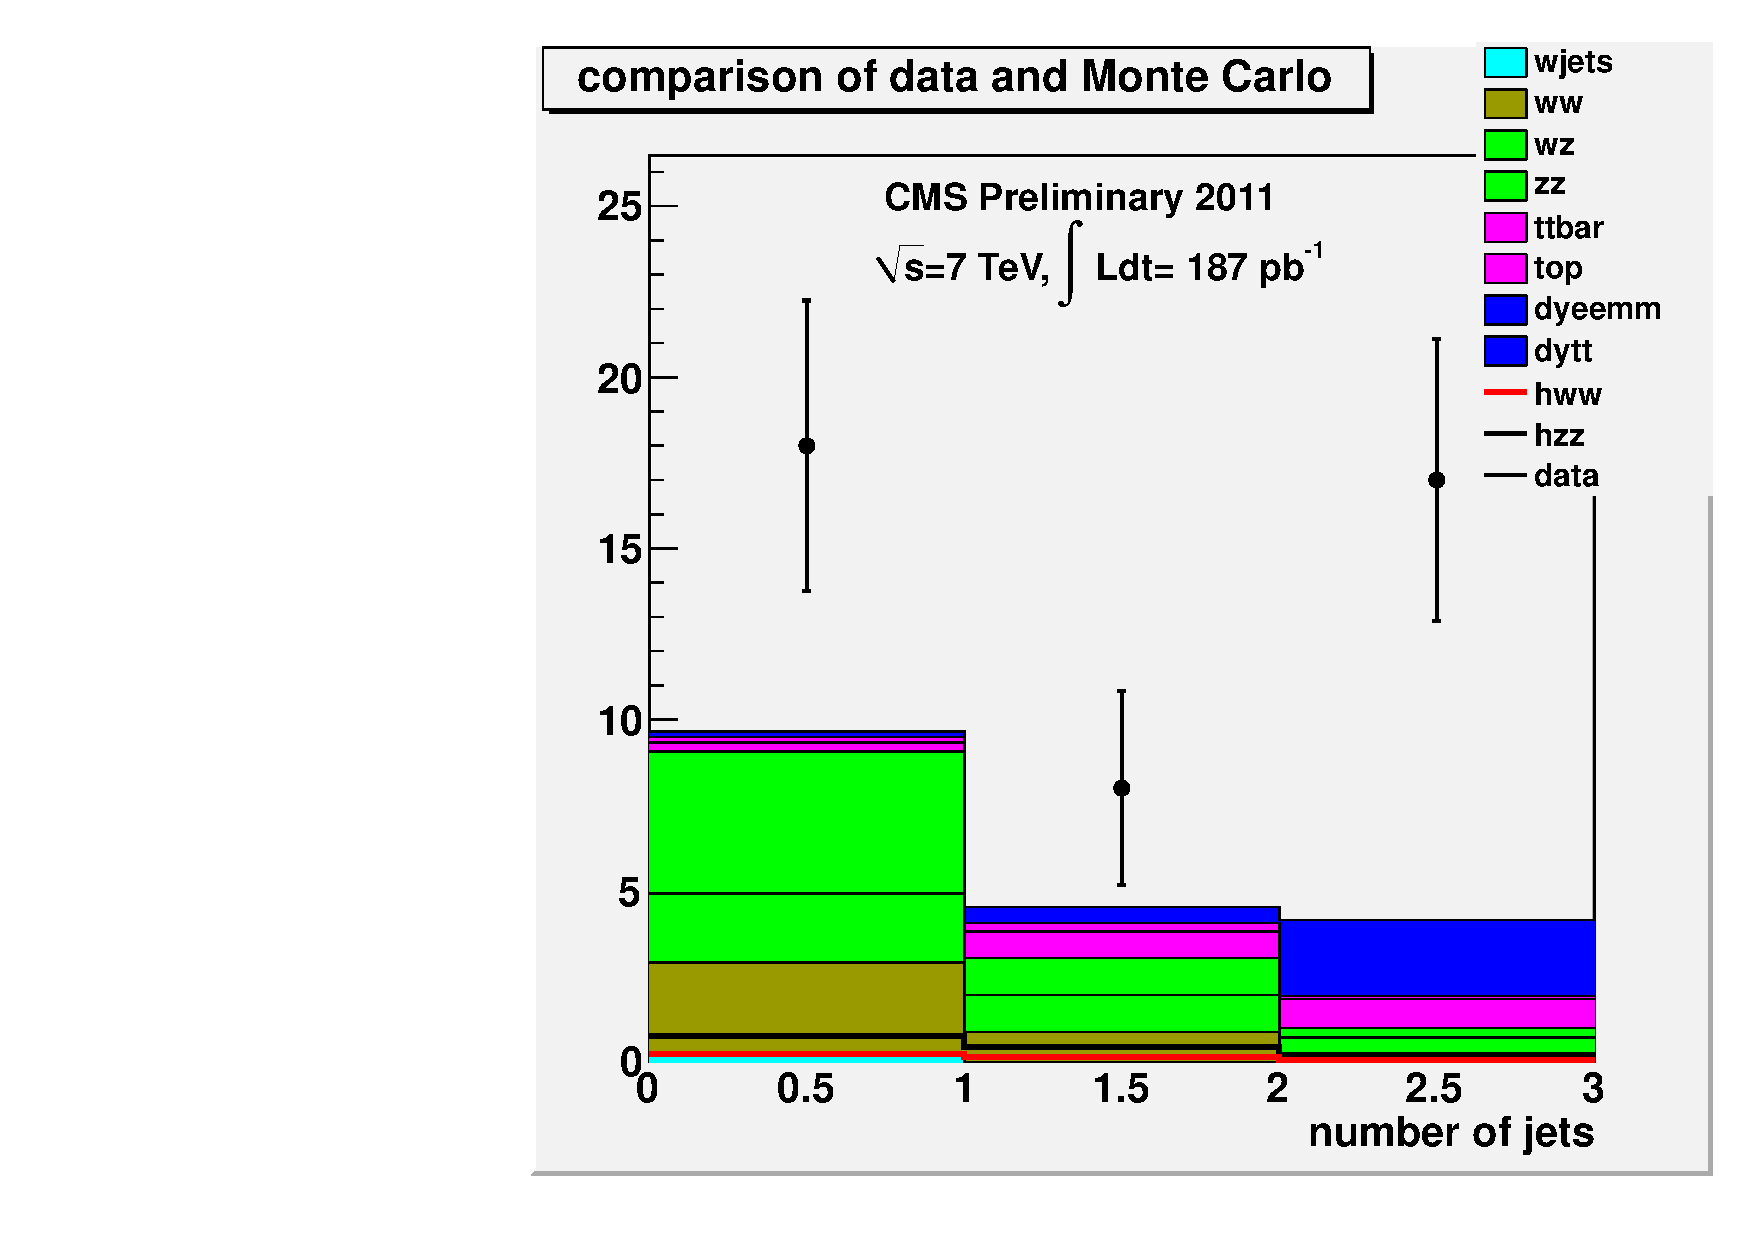
\includegraphics[width=.45\textwidth]{figures/preselection_njets.pdf}
\caption{Number of jets distribution observed in data corresponding to $187\pm7$~\ipb data, compared to the expected from simulation for signal and background. 
The background MC does not include any corrections, while we apply the $\pt$ reweighting correction in the higgs signal. }
\label{fig:njets_zzpresel}
\end{center}
\end{figure}
%%%%%%%%

%%%%%%%%
\begin{figure}[!hbtp]
\begin{center}
\label{fig:minmet_zzpresel}
\subfigure[0-Jet]{\label{subfig:minmet_0j}
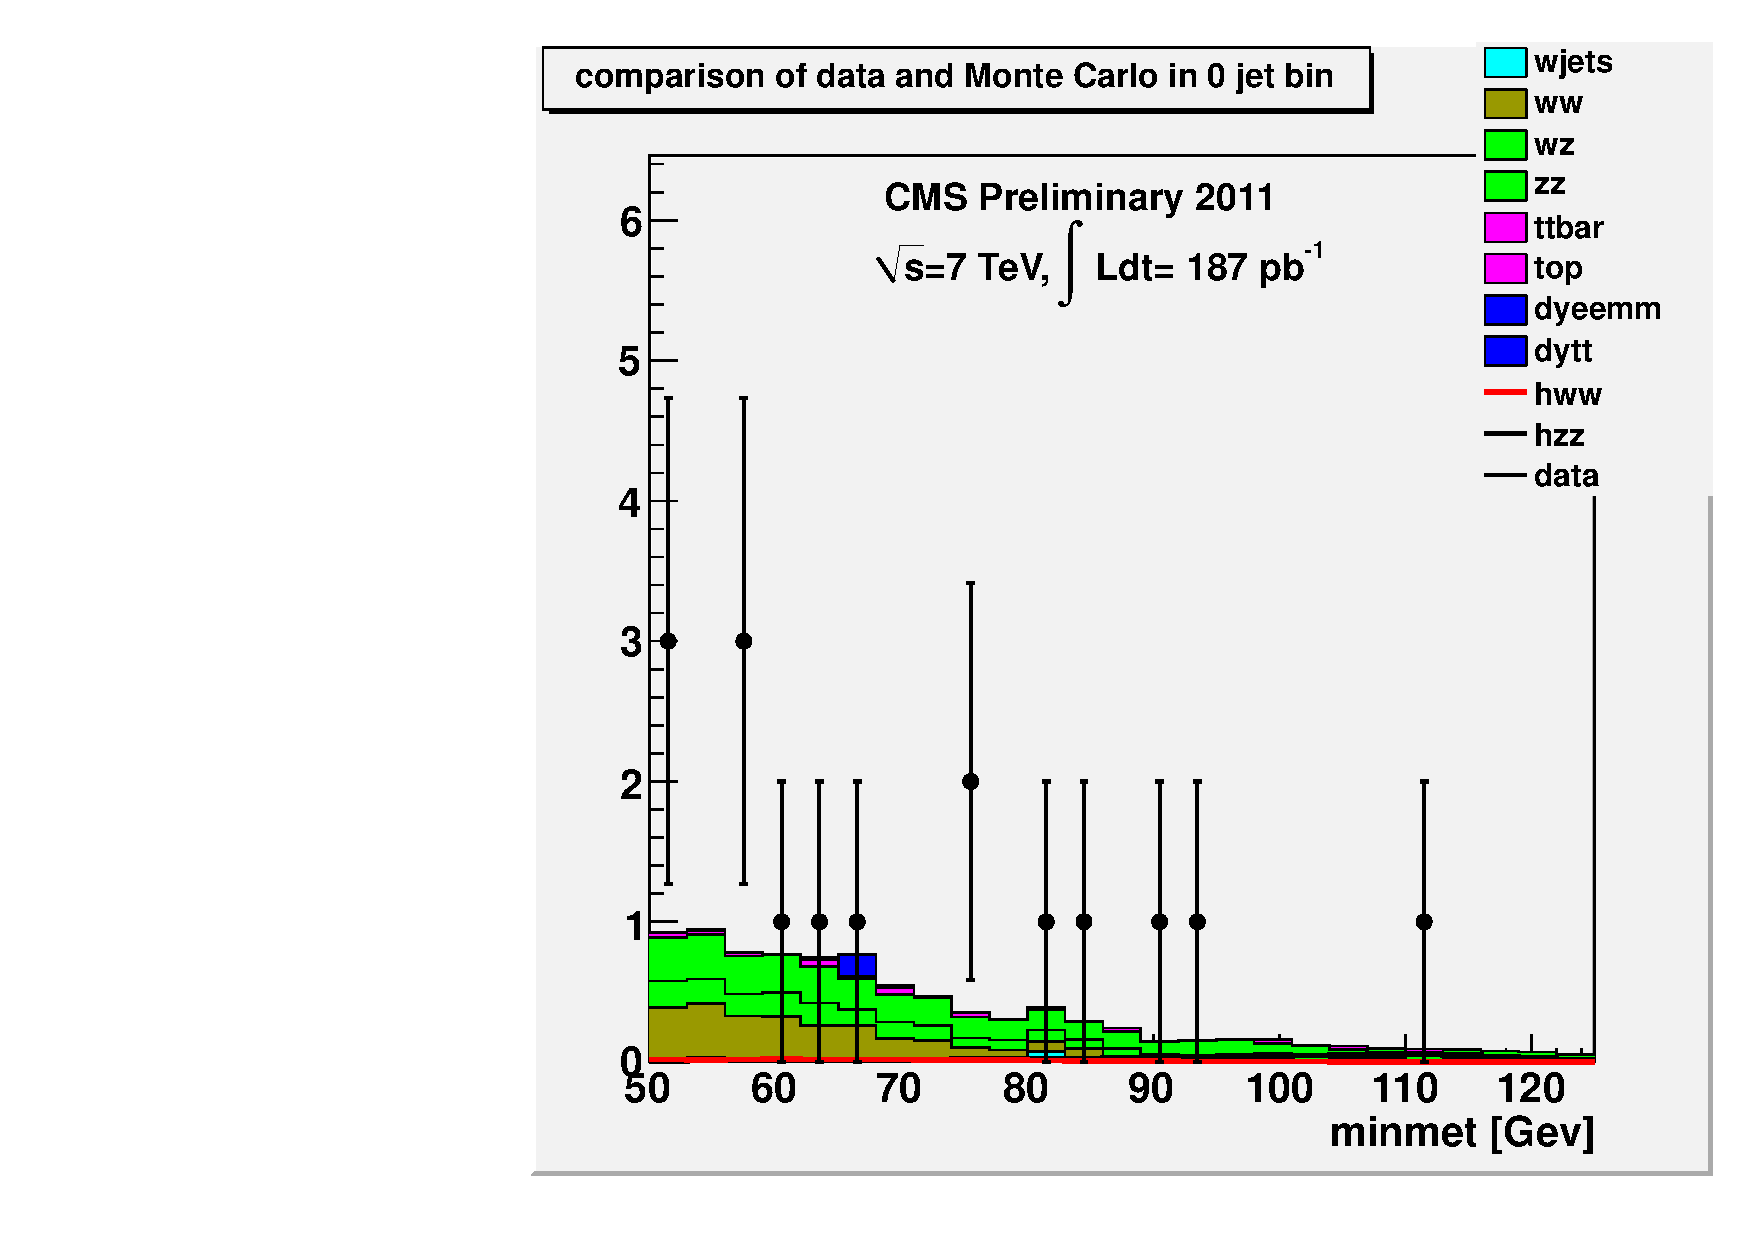
\includegraphics[width=.3\textwidth]{figures/preselection_0jets_minmet.pdf}}
\subfigure[1-Jet]{\label{subfig:minmet_1j}
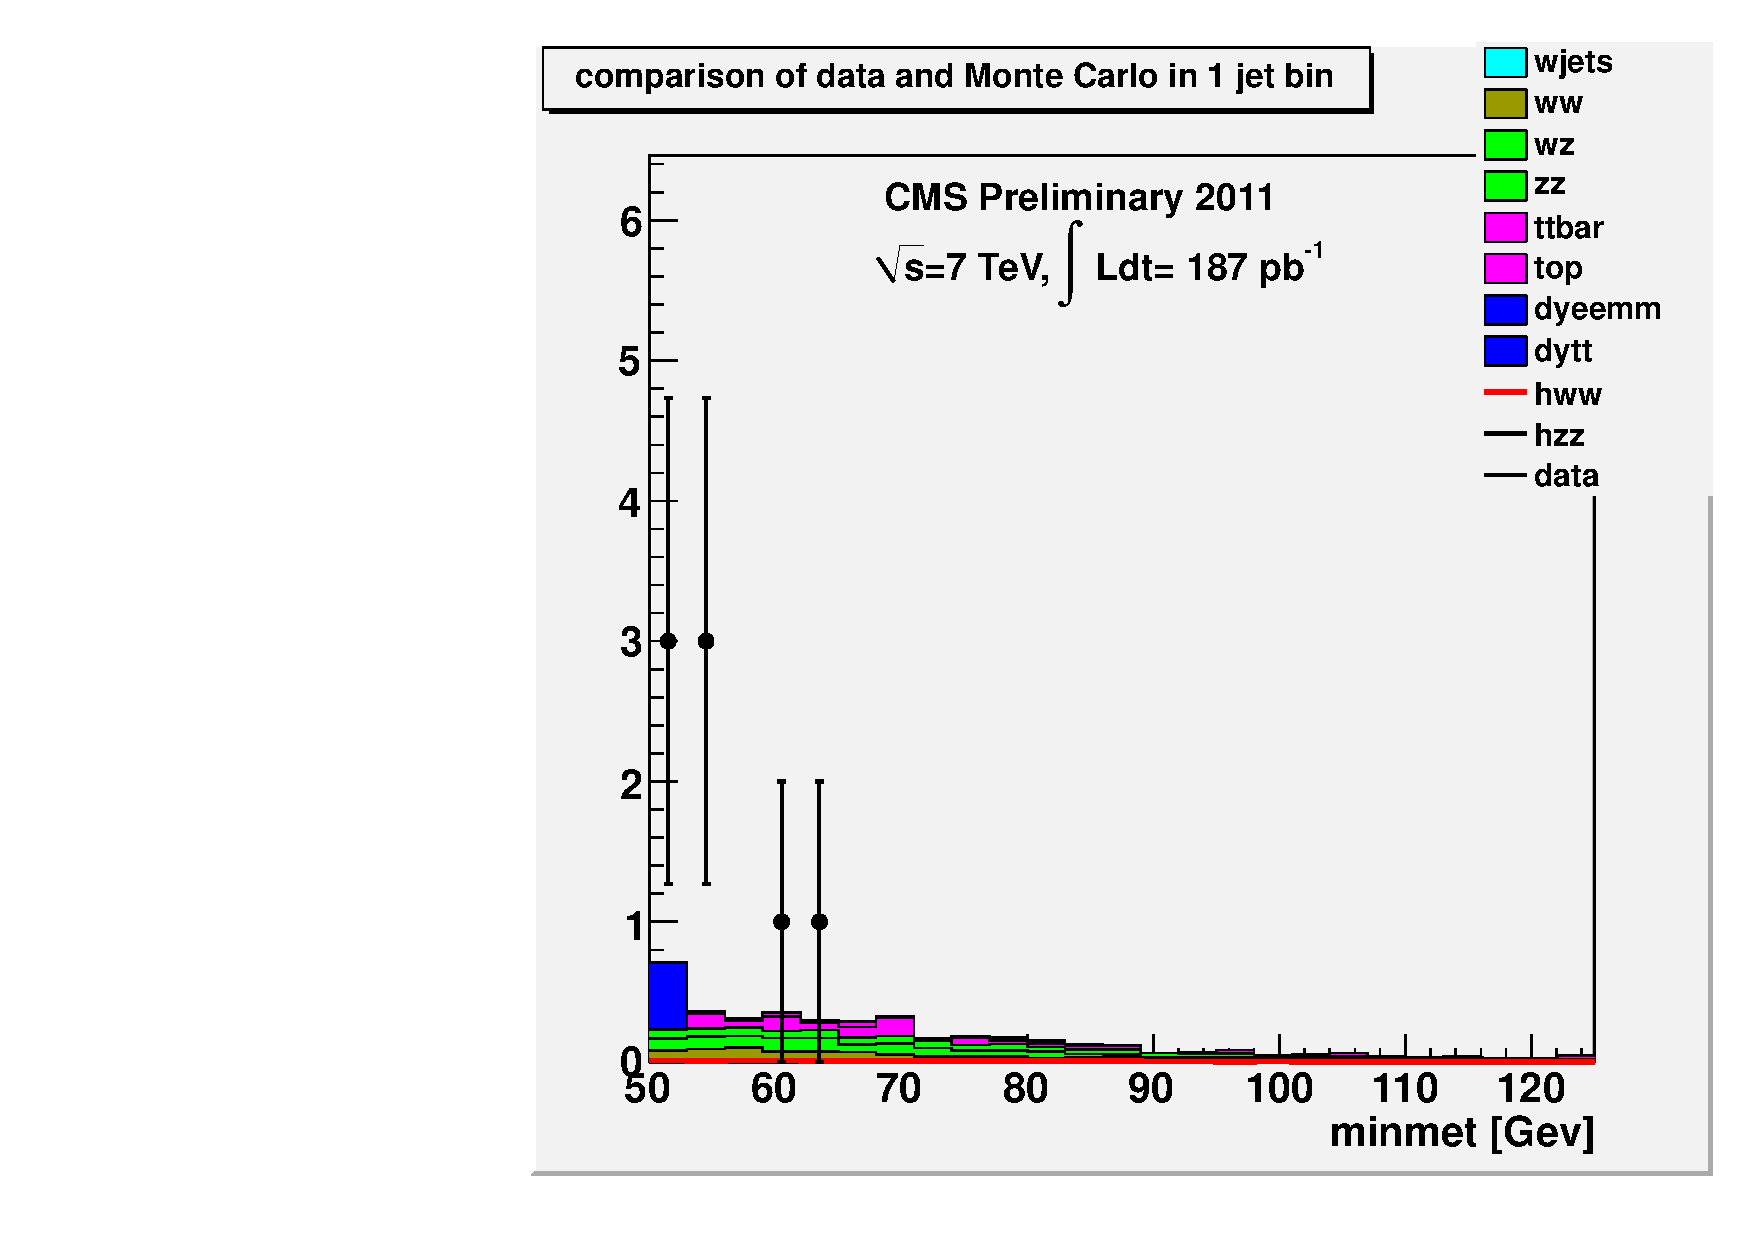
\includegraphics[width=.3\textwidth]{figures/preselection_1jet_minmet.pdf}}
\subfigure[$\geq$2 Jets]{\label{subfig:minmet_2j}
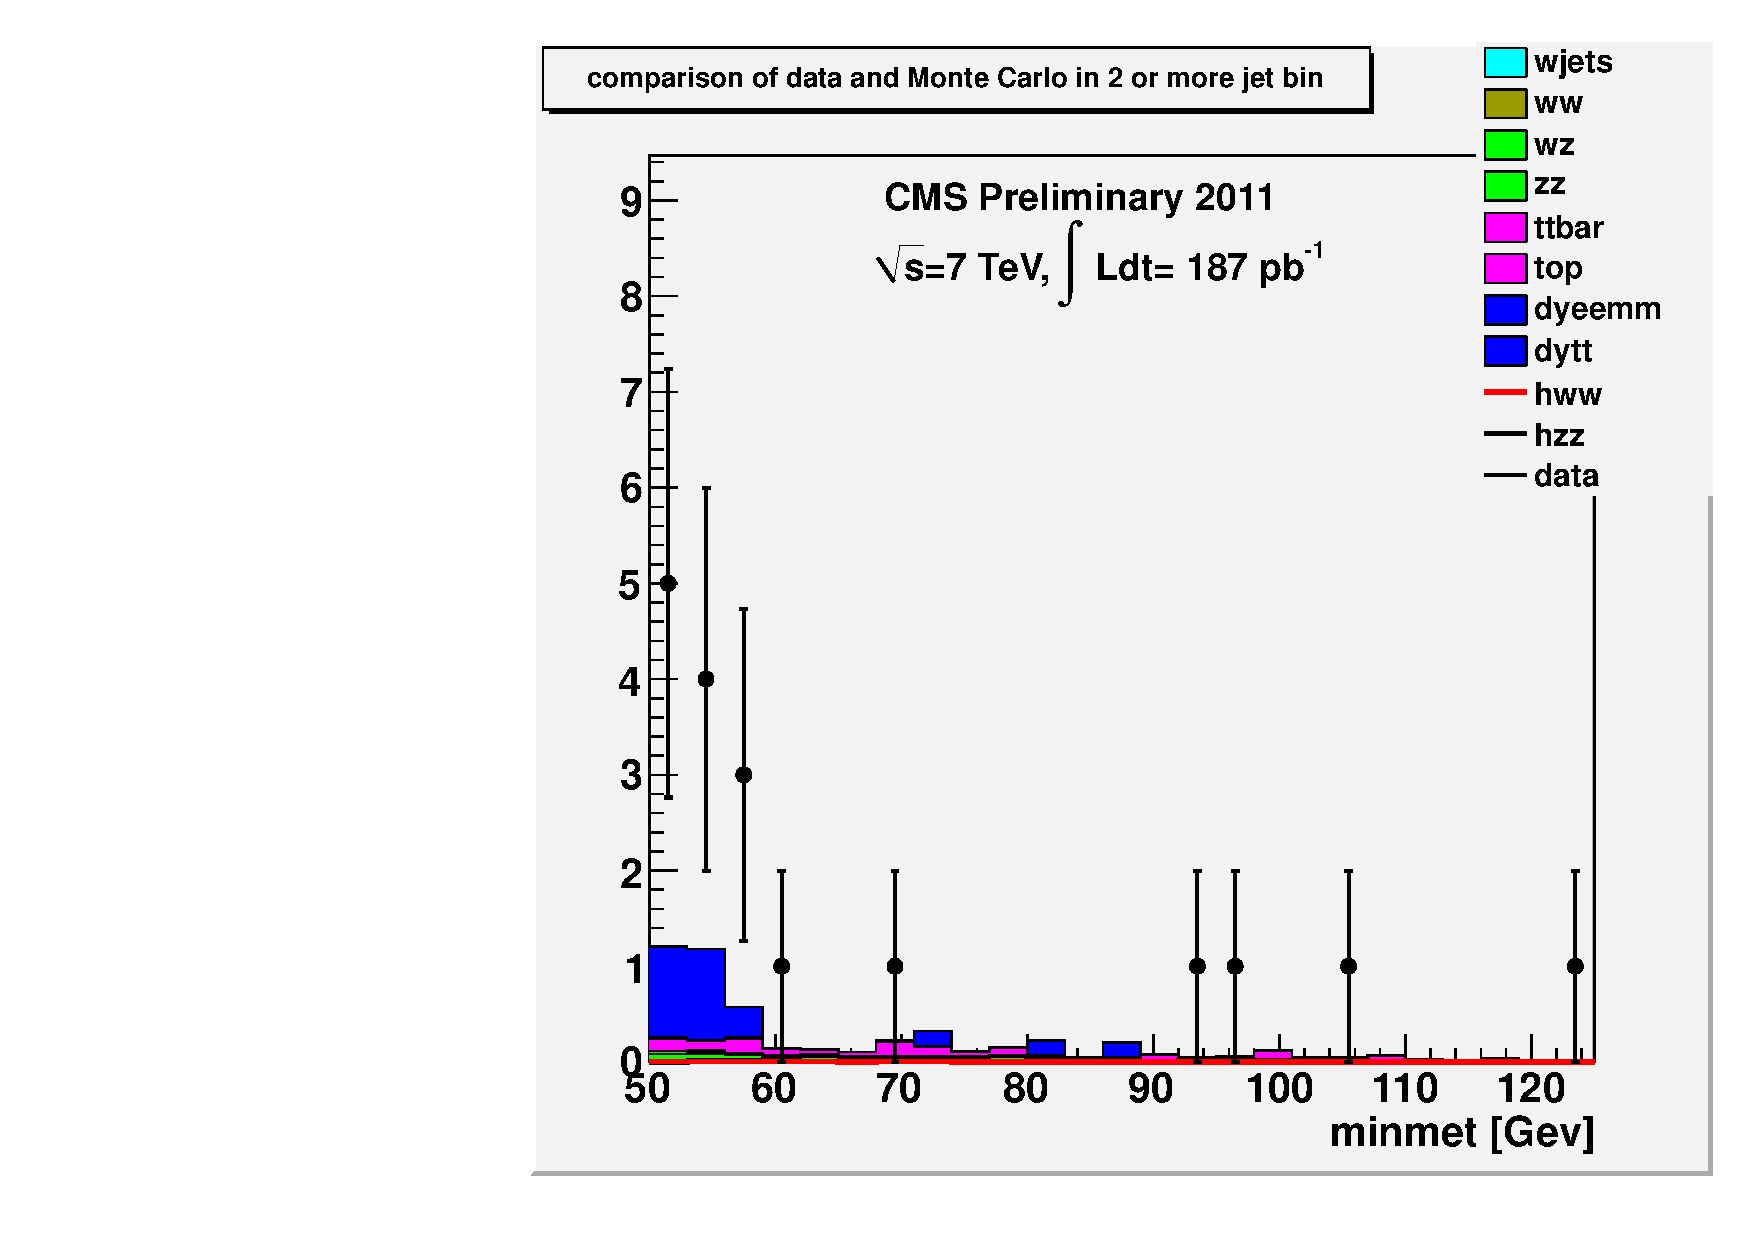
\includegraphics[width=.3\textwidth]{figures/preselection_2jets_minmet.pdf}}
\caption{Min-MET distribution after the $\ZZ$ preselection observed in data corresponding to $187\pm7$~\ipb data in 0-Jet~\subref{subfig:minmet_0j}, 1-Jet~\subref{subfig:minmet_1j} 
and 2-Jet~\subref{subfig:minmet_2j} bins, compared to the expected from simulation for signal and background. 
The background MC does not include any corrections, while we apply the $\pt$ reweighting correction in the higgs signal. }
\end{center}
\end{figure}
%%%%%%%%


%%%%%%%%
\begin{figure}[!hbtp]
\begin{center}
\label{fig:mt_zzpresel}
\subfigure[0-Jet]{\label{subfig:mt_0j}
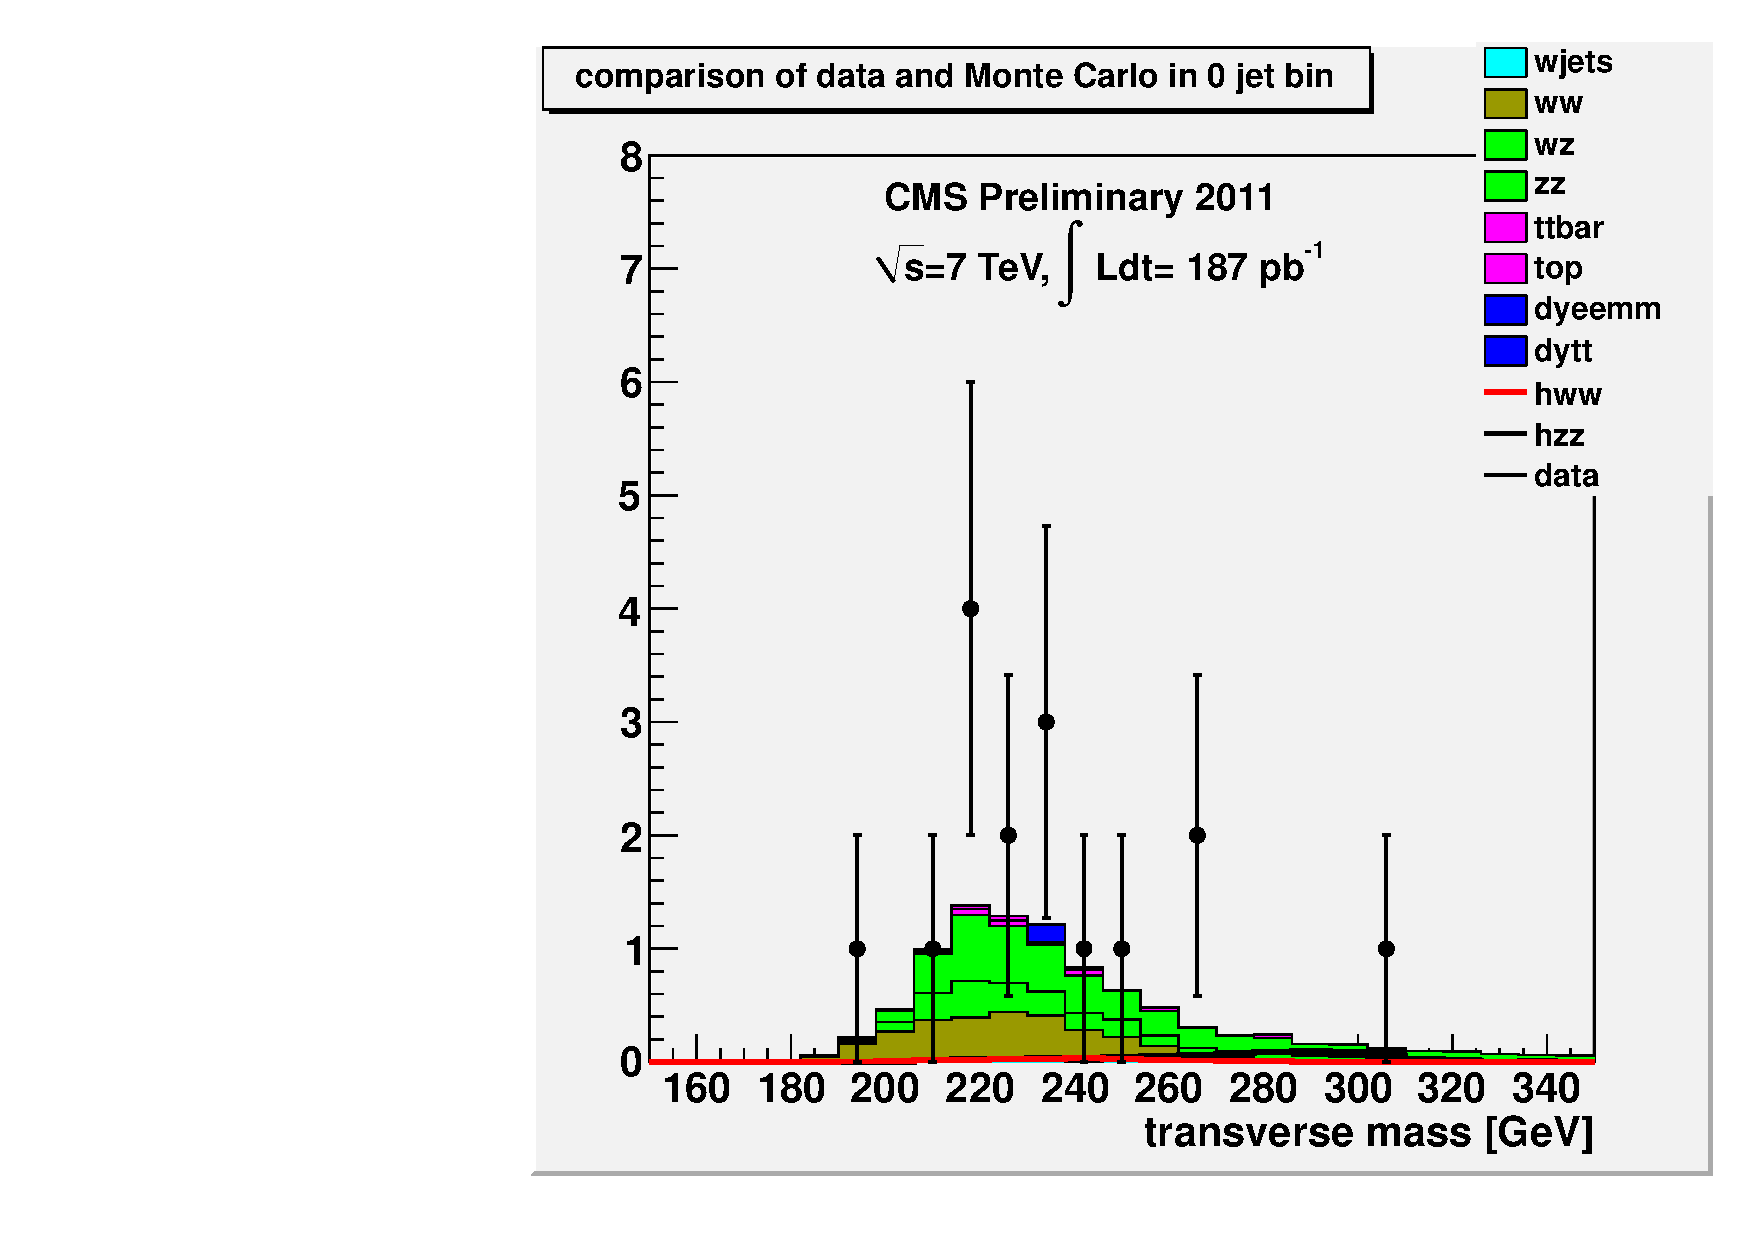
\includegraphics[width=.3\textwidth]{figures/preselection_0jets_mt.pdf}}
\subfigure[1-Jet]{\label{subfig:mt_1j}
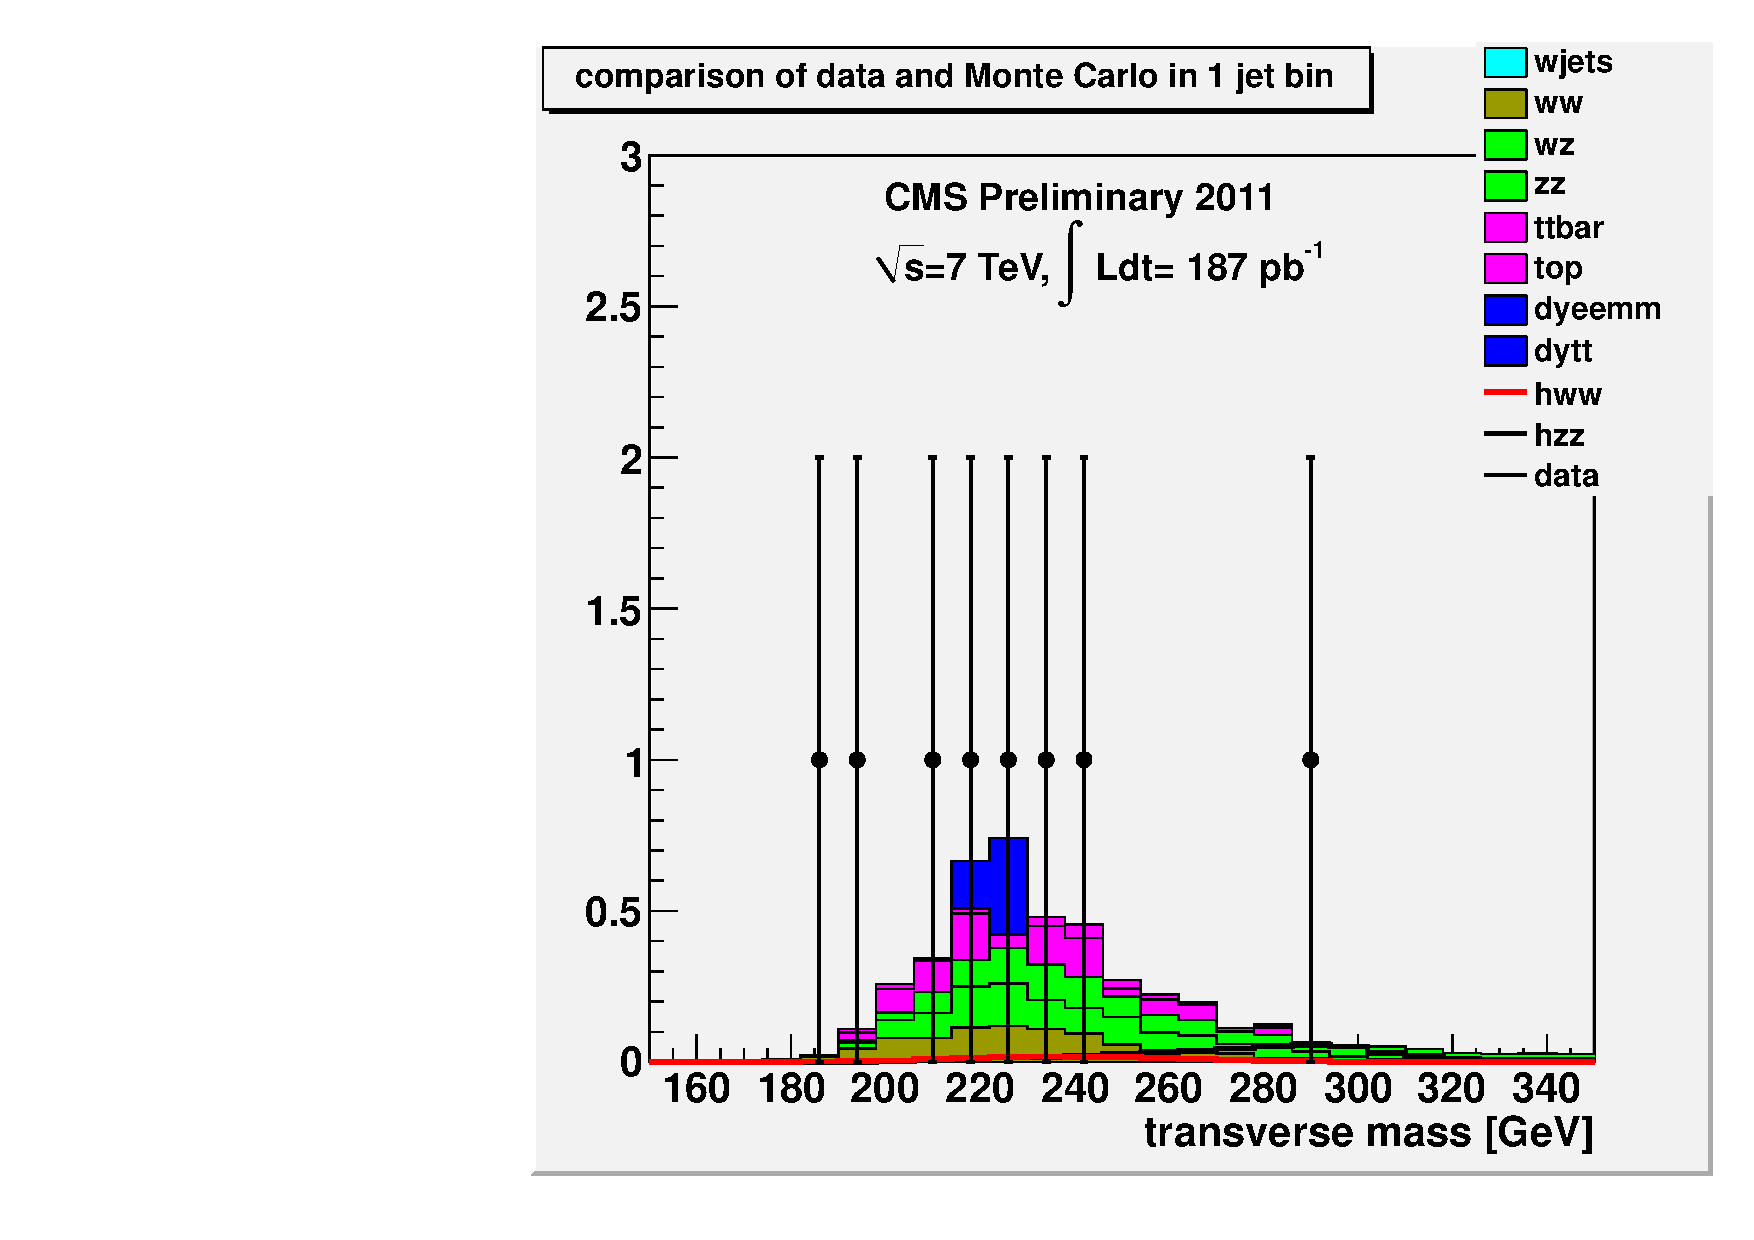
\includegraphics[width=.3\textwidth]{figures/preselection_1jet_mt.pdf}}
\subfigure[$\geq$2 Jets]{\label{subfig:mt_2j}
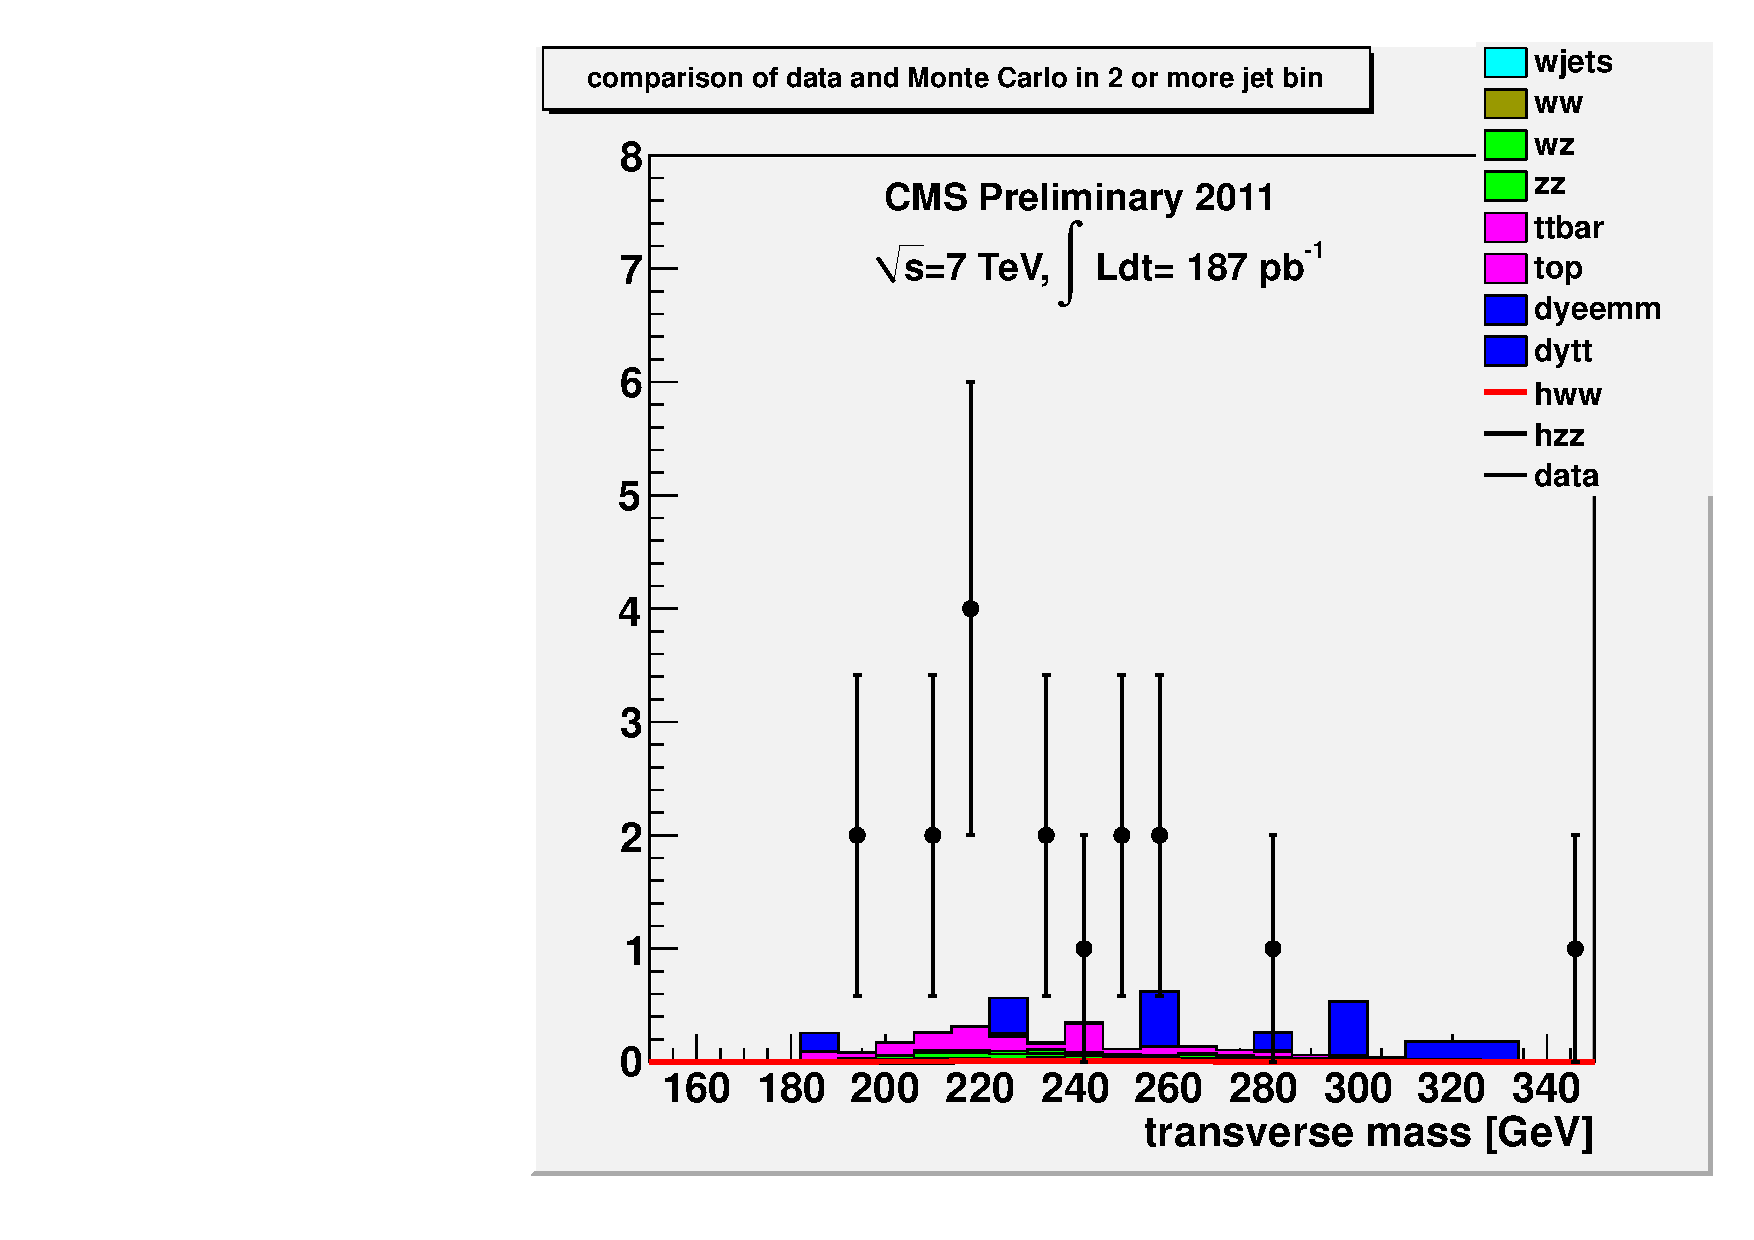
\includegraphics[width=.3\textwidth]{figures/preselection_2jets_mt.pdf}}
\caption{Transverse mass $m_T$ distribution after the $\ZZ$ preselection observed in data corresponding to $187\pm7$~\ipb data in 0-Jet~\subref{subfig:mt_0j}, 1-Jet~\subref{subfig:mt_1j} 
and 2-Jet~\subref{subfig:mt_2j} bins, compared to the expected from simulation for signal and background. 
The background MC does not include any corrections, while we apply the $\pt$ reweighting correction in the higgs signal. }
\end{center}
\end{figure}
%%%%%%%%

%%%%%%%%
\begin{figure}[!hbtp]
\begin{center}
\label{fig:mt_hzz300}
\subfigure[0-Jet]{\label{subfig:mt_0j}
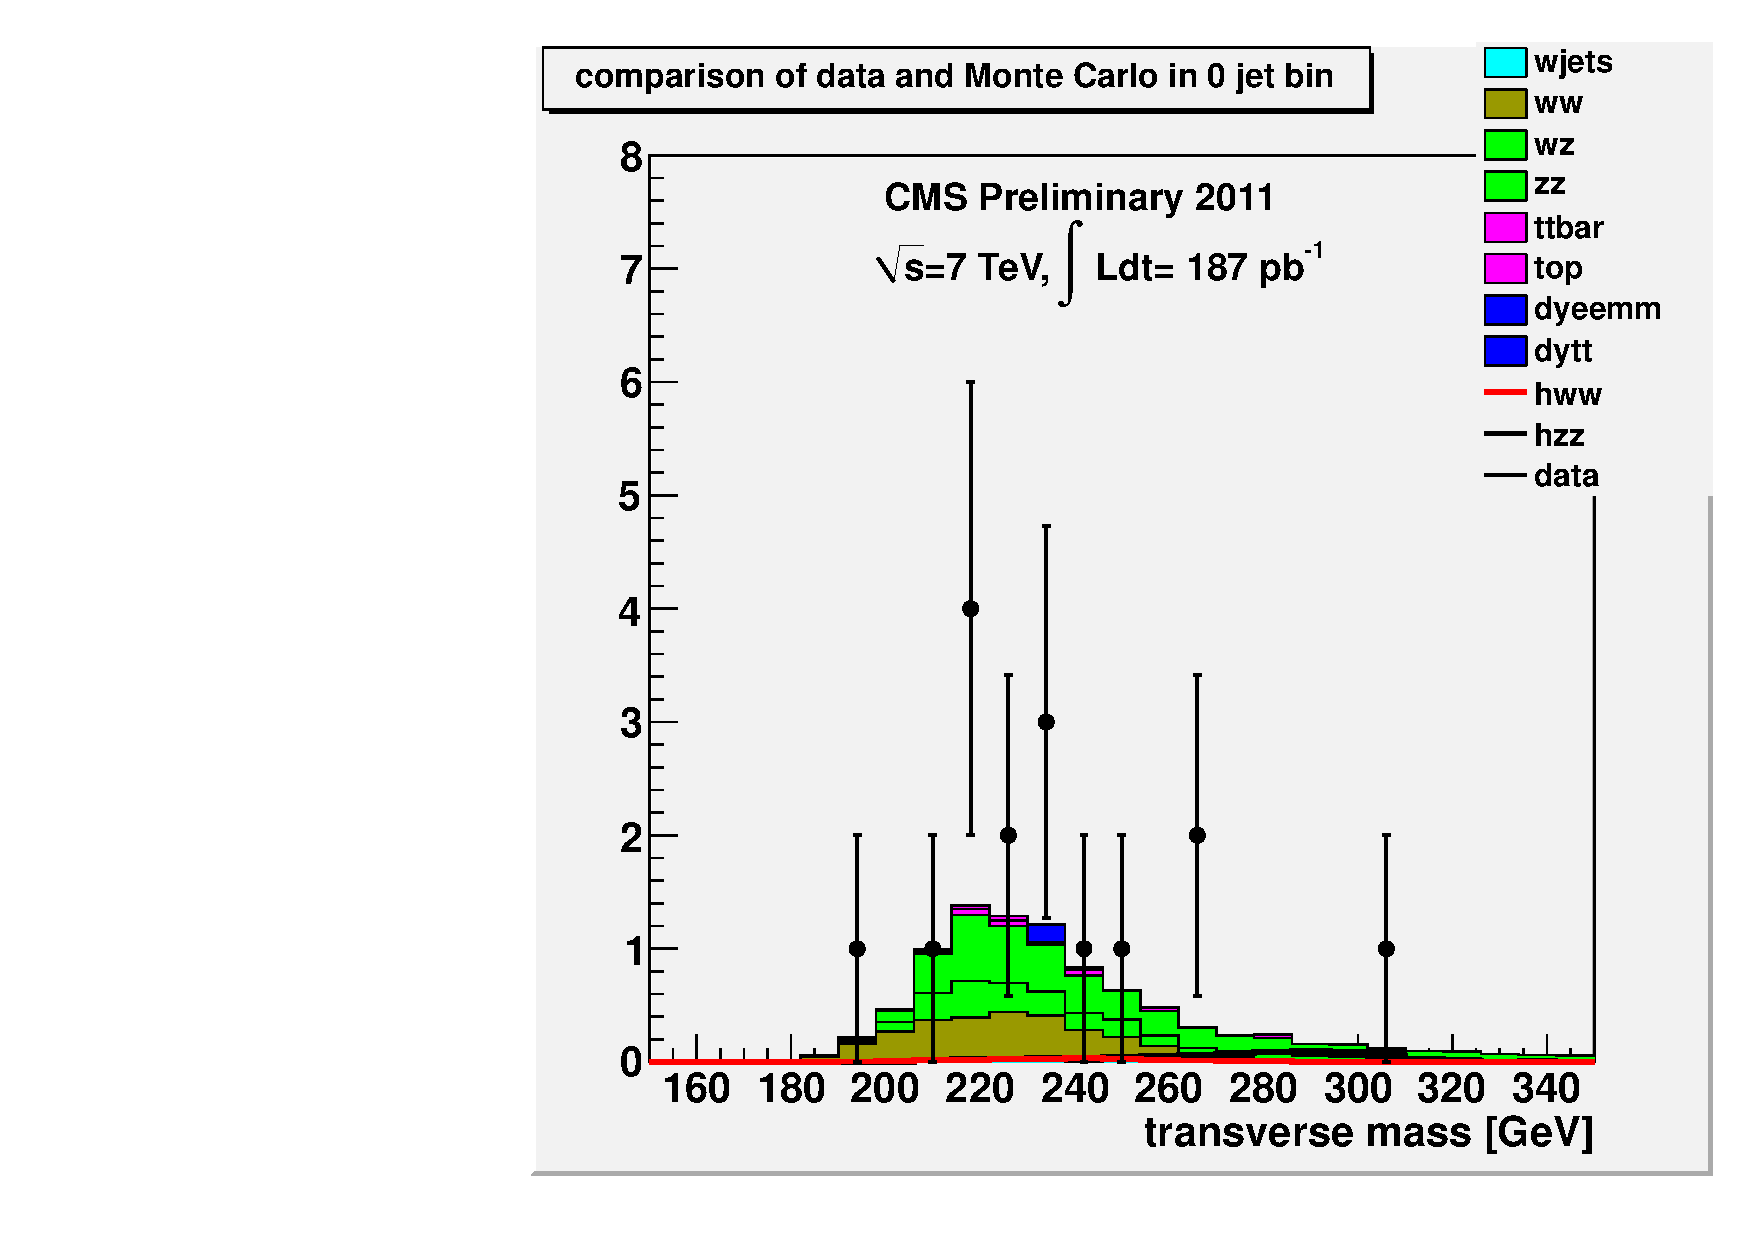
\includegraphics[width=.3\textwidth]{figures/preselection_0jets_mt.pdf}}
\subfigure[1-Jet]{\label{subfig:mt_1j}
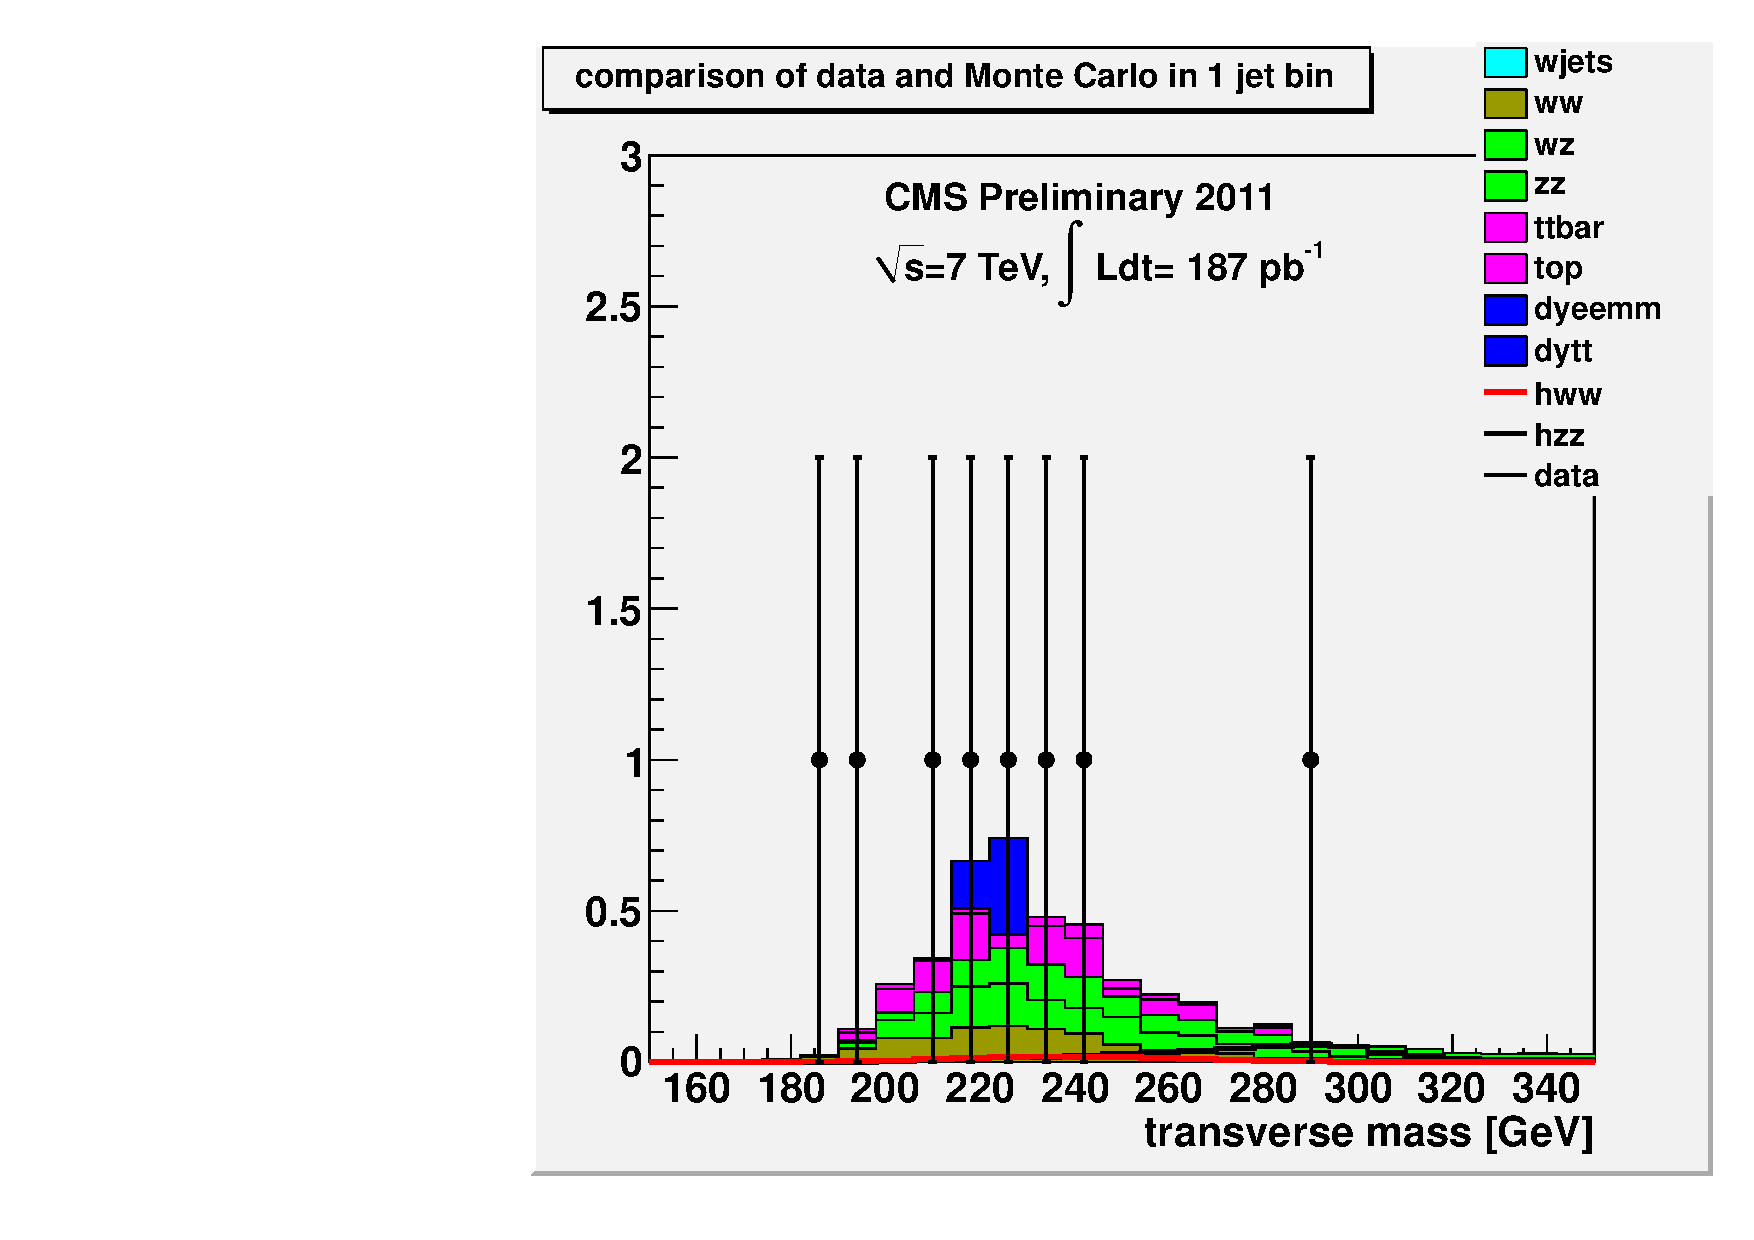
\includegraphics[width=.3\textwidth]{figures/preselection_1jet_mt.pdf}}
\subfigure[$\geq$2 Jets]{\label{subfig:mt_2j}
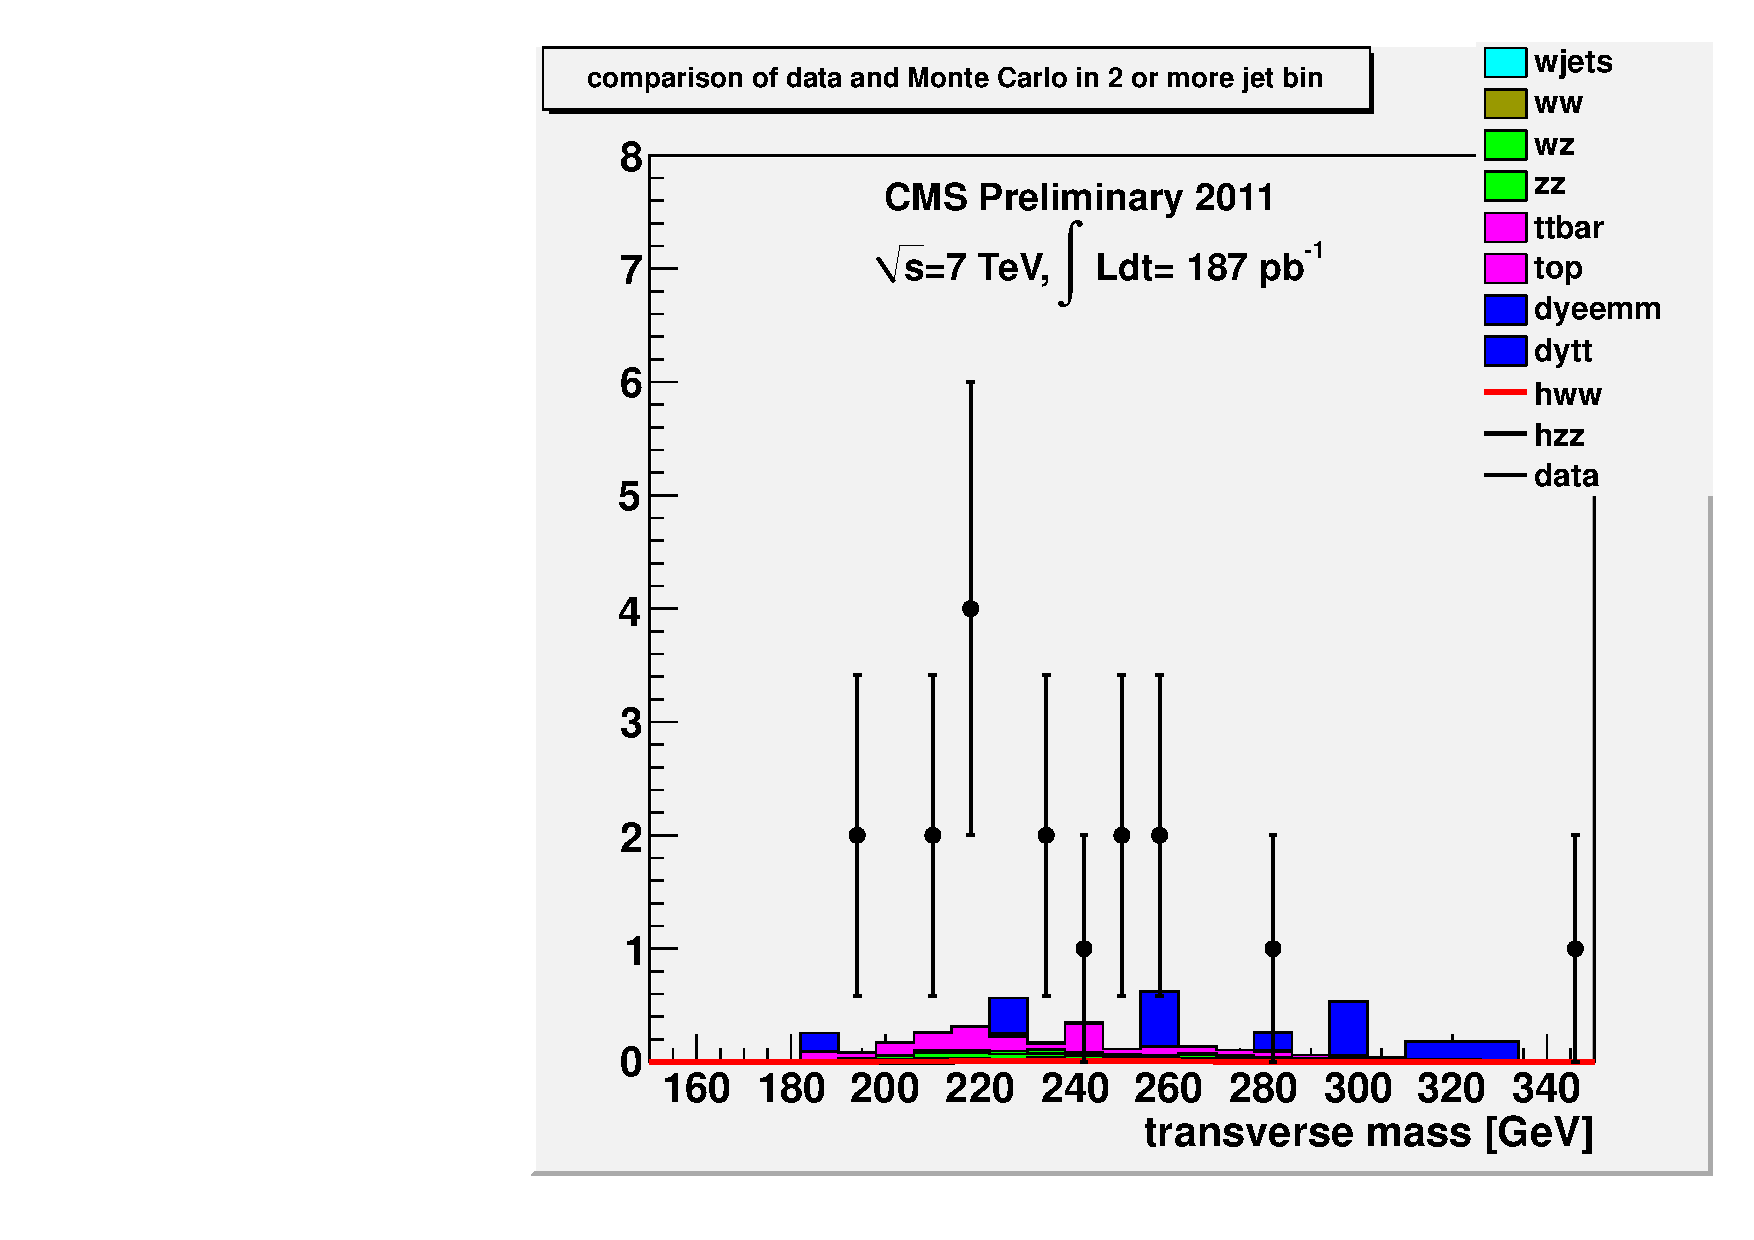
\includegraphics[width=.3\textwidth]{figures/preselection_2jets_mt.pdf}}
\caption{Transverse mass $m_T$ distribution after the full $\hzz$ ($m_H = 300\GeVcc$) selection observed in 
data corresponding to $187\pm7$~\ipb data in 0-Jet~\subref{subfig:mt_0j}, 1-Jet~\subref{subfig:mt_1j} 
and 2-Jet~\subref{subfig:mt_2j} bins, compared to the expected from simulation for signal and background. 
The background MC does not include any corrections, while we apply the $\pt$ reweighting correction in the higgs signal. }
\end{center}
\end{figure}
%%%%%%%%
